% A two-level oral-biofilm model from one variational principle: derivation, discretisation,
% verification, results and the rigour check.  Working note of the Keio continuation (P3);
% not part of the thesis.  Build: pdflatex unified_model.tex (twice).
% Sources: Klempt et al. 2024 (references/, Eq. 20-36), Klempt et al. 2026 (the point model, as
% coded in JAXFEM/core_hamilton_1d.py), Onsager's variational principle.  Nothing from
% F. Klempt's unpublished work.  Code: JAXFEM/unified_*.py, JAXFEM/fuel_front_*.py.
\documentclass[11pt,a4paper]{article}
\usepackage[margin=2.2cm]{geometry}
\usepackage{amsmath,amssymb,amsthm}
\usepackage{mathptmx}
\usepackage{booktabs,tabularx,array}
\usepackage{enumitem}
\usepackage[hyphens]{url}
\urlstyle{tt}
\usepackage{graphicx}
\graphicspath{{../assets/}}
\setlist{nosep,leftmargin=*}
\newcolumntype{Y}{>{\raggedright\arraybackslash}X}
\newtheorem{proposition}{Proposition}
\newtheorem{remark}{Remark}
\newcommand{\dd}{\,\mathrm{d}}
\newcommand{\D}{\mathrm{D}}
\newcommand{\living}{\textstyle\sum_i s_i\psi_i}
\title{\bfseries A two-level oral-biofilm model from one variational principle\\[2pt]
\large derivation, discretisation, verification and first results}
\author{Keisuke Nishioka}
\date{Working note, 15 October 2026 (Keio continuation; not part of the thesis)}
\begin{document}
\maketitle

\begin{abstract}
\noindent In the thesis the growth field of Klempt et al.\ 2024 and the multispecies point
model of Klempt et al.\ 2026 are solved separately and joined at the Gauss points, which needs
choices that no paper fixes: how the two voids relate, whether the point model is scaled to the
field, what drives the growth, and how the time of the point model is linked to the time of the field. Here the biofilm is described
on two levels, a phase field $\phi$ (biofilm against the outer liquid) and, inside the biofilm,
the composition of the point model, and all equations follow from one energy, one dissipation
potential and one constraint through the extended Hamilton principle in Onsager's form. Growth
is a reaction that consumes nutrient, catalysed by the living biomass. The model recovers the
point model where the field is uniform, the element's scheme (c) as its decoupled limit, and
the motion of the biofilm edge towards the nutrient without the front term of Klempt et al.\
2024. The total energy decreases along solutions. Every discrete equation solved is the
automatic derivative of the discrete functional, and the implementation is checked against the
point model to round-off. In 3D with the calibrated five-species point model, an antibiotic
lowers the living biomass, the growth and the advance of the edge, differently for a broad and
an anaerobe-specific antibiotic, and the composition varies with the local nutrient.
\end{abstract}

\section*{In plain words}

\paragraph{The problem.} In the thesis two models are computed separately and joined
afterwards: the field says where the biofilm is and how much of it there is, and the point
model says which species are inside and what fraction of each is alive. Joining them needs
choices that no paper makes: whether to scale the point model to the field (schemes (a) and
(b)), and what makes the biofilm grow (schemes (a) and (c)).

\paragraph{What is done here.} Both are written as one model from the start, and every
equation follows from one principle: the system moves so that its energy goes down, at a rate
set by friction (dissipation). Nothing is joined afterwards, so the choices above disappear.

\paragraph{What comes out.}
\begin{enumerate}
\item \emph{There are two kinds of empty space.} The liquid outside the biofilm and the liquid
  inside it are different things. A model that mixes them lets bacteria grow by themselves in
  the outer liquid.
\item \emph{Growth is a reaction that eats nutrient.} Living cells run it, so when an antibiotic
  kills cells, the growth slows down. Writing the living cells as the driver of the rate, not as
  an energy, is what makes the antibiotic work in the model.
\item \emph{The biofilm spreads towards the nutrient by itself.} Where there is more nutrient
  the biofilm grows more and pushes its edge out further. Klempt et al.\ 2024 added a separate
  term for this; here it follows from the growth, in 1D, 2D and 3D.
\end{enumerate}

\paragraph{In one sentence.} The thesis's scheme (c), growth from the living biomass, is the
simplest limit of this model, so it now has a derivation behind it.

\paragraph{How to read the rest.} Sections 1--5 give the model and its derivation, Section 6
the numerics, Section 7 the checks, Section 8 the results, Section 9 what is assumed and open.

\section{Why two levels}
\label{sec:two}

The direct generalisation of the point model to space takes every species as a field
$\phi_i(\mathbf X,t)$ with one void $\phi_0=1-\sum_i\phi_i$ and the point-model energy at every
point. The point model keeps every $\phi_i$ away from zero by its barrier energy
$K/[\phi_i^2(1-\phi_i)^2]$, and its production is local. Solved in 1D with all fields in one
Newton system (\path{unified_1d_monolithic.py}), the outer liquid fills up from the barrier
floor everywhere at once (at $T^*=1$ the amount far from the seed had risen from $0.05$ to
$0.43$), so the model cannot represent a biofilm next to liquid. The two voids are therefore
different physical objects: the liquid outside the biofilm, which the field of Klempt et al.\
2024 describes, and the liquid inside it, which the point model's $\phi_0$ describes. The model
below keeps both.

\section{State}

\begin{center}
\begin{tabular}{@{}lll@{}}
\toprule
symbol & meaning & source\\
\midrule
$\phi(\mathbf X,t)\in[0,1]$ & biofilm phase: biofilm against the outer liquid & Klempt et al.\ 2024\\
$s_i(\mathbf X,t)$, $i=1\dots n$ & share of species $i$ in the biofilm & Klempt et al.\ 2026 ($\phi_i$ there)\\
$s_0(\mathbf X,t)$ & inner liquid, $\sum_is_i+s_0=1$ & Klempt et al.\ 2026 ($\phi_0$ there)\\
$\psi_i(\mathbf X,t)$ & living fraction of species $i$ & Klempt et al.\ 2026\\
$\gamma(\mathbf X,t)$ & multiplier of the composition constraint & Klempt et al.\ 2026\\
$c(\mathbf X,t)$ & nutrient concentration & Klempt et al.\ 2024\\
$\alpha(\mathbf X,t)$ & local expansion, $\mathbf F_g=\alpha\mathbf I$, $\alpha(0)=1$ & Klempt et al.\ 2024\\
$\mathbf u(\mathbf X,t)$ & displacement & Klempt et al.\ 2024\\
\bottomrule
\end{tabular}
\end{center}
The absolute amount of species $i$ is $\phi s_i$ and the living biomass is $\phi\living$. The
point model's $\bar\phi_i=\phi_i\psi_i$ is $s_i\psi_i$ here. All fields live in the reference
configuration $\mathbf X$.

\section{Energy, dissipation, constraint}

Let $h(\phi)=\phi^2$ be the weight with which the biofilm carries its composition, and
$w=h(\phi)+\varepsilon$ with a small $\varepsilon>0$ that keeps the composition equations
regular in the outer liquid, where they carry no weight.

\paragraph{Composition.} The energy of the point model of Klempt et al.\ 2026, per unit
biofilm,
\begin{equation}
\Psi_{\rm pm}=\underbrace{K\Big[\sum_iB(s_i)+B(s_0)+\sum_iB(\psi_i)\Big]}_{\Psi_{\rm bar}}
+\underbrace{\frac{\alpha^*}{2}\sum_ib_i\psi_i^2-\frac{c^*}{2}\sum_{ij}A_{ij}\,s_i\psi_i\,s_j\psi_j}_{\Psi_{\rm int}},
\qquad B(x)=\frac{1}{x^2(1-x)^2},
\label{eq:pm}
\end{equation}
with the barrier constant $K=10^{-4}$, the interaction matrix $A$ (calibrated, symmetric), the
nutrient constant $c^*$, the antibiotic concentration $\alpha^*$ and the susceptibilities
$b_i$. The barrier terms keep $s_i,s_0,\psi_i$ inside $(0,1)$. Both parts are stored energy
and carry the weight $w$ (Remark~\ref{rem:barrier}).

\paragraph{Phase, nutrient, growth.} With the gradient energies of Klempt et al.\ 2024, a
one-sided barrier that keeps $\phi\le1$, the free energy of an ideal solute for the nutrient
and the chemical potential $\mu_b$ of grown biomass,
\begin{equation}
E=\frac{\beta}{2}|\nabla\phi|^2+\frac{K_\phi}{(1-\phi)^2}
+\lambda w\,\Psi_{\rm pm}+w\frac{\beta_s}{2}\sum_i|\nabla s_i|^2
+c(\ln c-1)+\mu_b\,\xi+E_{\rm mech},\qquad \xi=\alpha-1 .
\label{eq:E}
\end{equation}
$\lambda$ is the energy scale of the composition relative to the phase, $\beta_s$ the
spreading of the composition inside the biofilm, and $E_{\rm mech}=\tfrac{\mu}{2}\phi^2
(\mathbf I:\mathbf C_e-3)$ the mechanical energy of Klempt et al.\ 2024, which does not enter
the growth equations (as there: its effect on growth is small).

\paragraph{Dissipation.} Quadratic in the rates, from Klempt et al.\ 2026 for the composition
and Klempt et al.\ 2024 for the phase, and for the two fluxes of the growth reaction:
\begin{equation}
\D=\frac{\eta_\phi}{2}\dot\phi^2+\lambda w\,\D_{\rm pm}+\frac{\dot\xi^2}{2L}+\frac{|\mathbf j|^2}{2Dc},\qquad
\D_{\rm pm}=\sum_i\Big[\frac{\eta}{2}\dot s_i^2+\frac{\eta}{2}\big(\tfrac{\dd}{\dd t}(s_i\psi_i)\big)^2\Big]+\frac12\dot s_0^2 ,
\label{eq:D}
\end{equation}
where $\mathbf j$ is the nutrient flux and $L$ the mobility of the growth reaction. The living
biomass is its catalyst,
\begin{equation}
L=L_0\,\phi\living ,
\label{eq:L}
\end{equation}
so lysis or an antibiotic lowers the growth through the mobility and exerts no force on
$\psi_i$ (Remark~\ref{rem:catalyst}).

\paragraph{Constraints.} The composition constraint with the multiplier field,
$\lambda w\gamma(\sum_is_i+s_0-1)$, and the balance of the growth reaction, which turns $Y$
units of nutrient into one unit of growth,
\begin{equation}
\dot c+Y\dot\xi+\nabla\!\cdot\mathbf j=0 .
\label{eq:balance}
\end{equation}

\section{The principle and the evolution equations}

For the state $q=\{\phi,s_i,s_0,\psi_i,\gamma\}$ the extended Hamilton principle of Junker
and Balzani (as used by Klempt et al.\ 2024) states
\begin{equation}
\delta_q\int_\Omega E\dd V+\int_\Omega\frac{\partial\D}{\partial\dot q}\,\delta q\dd V=0
\qquad\forall\,\delta q,
\label{eq:principle}
\end{equation}
with $\mathbf n\cdot\nabla\phi=\mathbf n\cdot\nabla s_i=0$ on the boundary; the dissipation is
varied with respect to the rates only. For the reaction and the flux it is Onsager's form:
$\dot\xi$ and $\mathbf j$ minimise the Rayleighian $\frac{\dd}{\dd t}\int E+\int\D$ under the
balance \eqref{eq:balance}.

\paragraph{Composition} (each equation divided by $\lambda w>0$):
\begin{align}
KB'(s_i)+\gamma+\eta(1+\psi_i^2)\dot s_i+\eta s_i\psi_i\dot\psi_i-c^*\psi_i\sum_jA_{ij}s_j\psi_j
-\frac{\beta_s}{\lambda w}\nabla\!\cdot(w\nabla s_i)&=0,\label{eq:s}\\
KB'(s_0)+\gamma+\dot s_0&=0,\\
KB'(\psi_i)+\alpha^*b_i\psi_i+\eta s_i\psi_i\dot s_i+\eta s_i^2\dot\psi_i-c^*s_i\sum_jA_{ij}s_j\psi_j&=0,\label{eq:psi}\\
\textstyle\sum_is_i+s_0-1&=0 .
\end{align}
Without the gradient term these are the point model of Klempt et al.\ 2026 at every point, in
its own time.

\paragraph{Phase:}
\begin{equation}
\eta_\phi\dot\phi-\beta\nabla^2\phi+\frac{2K_\phi}{(1-\phi)^3}
+\lambda h'(\phi)\Psi_{\rm pm}+h'(\phi)\frac{\beta_s}{2}\sum_i|\nabla s_i|^2=0 .
\label{eq:phi}
\end{equation}
The composition acts on the phase through $\lambda h'(\phi)\Psi_{\rm pm}$: where the
composition energy is low (strong favourable interactions) the biofilm tends to grow, where it
is high (an antibiotic, $\alpha^*b_i\psi_i^2/2$) it tends to recede. Because $h'(0)=0$, the
composition exerts no force where there is no biofilm.

\paragraph{Growth and nutrient.} With $\mu_c=\partial_cE=\ln c$, the Rayleighian under
\eqref{eq:balance} gives
\begin{equation}
\dot\xi=L\,(Y\ln c-\mu_b),\qquad \mathbf j=-D\nabla c,\qquad
\dot c=D\nabla^2c-Y\dot\xi ,
\label{eq:growth}
\end{equation}
with $c=1$ on the supplying boundary and $\mathbf n\cdot\nabla c=0$ elsewhere. Writing
$\mu_b=Y\ln c_{\rm stop}$, growth stops where $c$ falls to $c_{\rm stop}$. The kinematics is
that of Klempt et al.\ 2024, $\mathbf F=\mathbf F_e\mathbf F_g$, $\mathbf F_g=\alpha\mathbf I$.

\paragraph{Mechanics.} The principle of virtual work with the stiffness
$(\phi^2+f)E_{\rm bio}$ of Klempt et al.\ 2024, unchanged.

\begin{remark}[the barrier terms]\label{rem:barrier}
In the one-level point model only the derivatives of $\Psi_{\rm bar}$ matter. Weighted with
the biofilm amount, its value also acts on the phase, $\lambda h'(\phi)\Psi_{\rm bar}$. At the
calibration's start ($\psi_i=0.999$) this value is about $500$, against about $8$ for the
interactions; after the initial transient ($\psi_i\approx0.9$) it is below $0.1$. Two
alternatives were tried, holding the barrier weight fixed (a regularised constraint) and giving
it a constant weight; both change $\alpha$ by about $6\,\%$ and the first breaks the exact
energy inequality. The literal form, barrier terms as stored energy with the weight $w$, is
kept: it is what Klempt et al.\ 2026 wrote, and it makes Proposition~\ref{prop:energy} exact.
\end{remark}

\begin{remark}[growth energy or growth reaction]\label{rem:catalyst}
A first version drove the growth by an energy $-k_\alpha(\alpha-1)\phi\living$, which gives
$\dot\alpha=k_\alpha\phi\living$ directly. Its derivative with respect to $\psi_i$ is a force
that keeps cells alive where growth has happened; at large growth it defeats an antibiotic
(at $k_\alpha=8$ the antibiotic lowered the growth by $0.7\,\%$ only). The reaction form
\eqref{eq:growth}--\eqref{eq:L} puts the living biomass into the mobility, where it belongs:
a catalyst changes the rate, not the energy. It also replaces $k_\alpha$ by quantities with a
meaning ($L_0$, $Y$, $c_{\rm stop}$) and makes the energy inequality include the nutrient.
\end{remark}

\section{Properties}

\begin{proposition}[energy inequality]\label{prop:energy}
Let $E$ not depend on time explicitly and let the boundary be closed ($\mathbf n\cdot\mathbf
j=0$). Along solutions of \eqref{eq:s}--\eqref{eq:growth},
\[\frac{\dd}{\dd t}\int_\Omega E\dd V=-\int_\Omega\Big[2\lambda w\D_{\rm pm}+\eta_\phi\dot\phi^2
+\frac{\dot\xi^2}{L}+\frac{|\mathbf j|^2}{Dc}\Big]\dd V\le0 .\]
\end{proposition}
\begin{proof}
Multiply each stationarity condition of \eqref{eq:principle} by its rate, integrate and add.
The gradient terms integrate by parts to the rates of the gradient energies (the boundary terms
vanish by the no-flux conditions), the constraint terms give $\lambda w\gamma\frac{\dd}{\dd
t}(\sum_is_i+s_0)=0$, and $\D_{\rm pm}$ and $\dot\phi^2$ are quadratic in the rates, so the
rates times the dissipative forces give twice the dissipation. For the reaction,
$\partial_cE\,\dot c+\mu_b\dot\xi=\mu_c(-Y\dot\xi-\nabla\!\cdot\mathbf j)+\mu_b\dot\xi
=-(Y\mu_c-\mu_b)\dot\xi+\mathbf j\cdot\nabla\mu_c$ after integration by parts, and
\eqref{eq:growth} gives $Y\mu_c-\mu_b=\dot\xi/L$ and $\nabla\mu_c=-\mathbf j/(Dc)$.
\end{proof}

\begin{remark}
A supplying boundary ($c=1$) and a switch of the antibiotic ($\alpha^*$ changing in time) are
external inputs: the first adds the inflow of nutrient energy, the second
$\int\lambda w\,\tfrac12\dot\alpha^*\sum_ib_i\psi_i^2$. Both appear in the computations as the
only increases of the discrete energy.
\end{remark}

\paragraph{Limits.}
\begin{enumerate}
\item Uniform field, $\beta_s=0$: at every point the composition is the point model of Klempt
  et al.\ 2026 in its own time. The calibrated $A$, $c^*$ and the time link of the calibration
  carry over unchanged.
\item $\lambda\to0$, $\beta_s=0$: the composition decouples from the phase and runs where the
  biofilm is, as the element's free point model (scheme (b)); the growth
  $\dot\alpha=L_0\phi\living\,(Y\ln c-\mu_b)$ is the element's scheme (c),
  $\dot\alpha=\kappa\,\phi_{3D}\sum_i\bar\phi_i$, with $\kappa=L_0(Y\ln c-\mu_b)$. Scheme (c)
  is thus the decoupled limit of this model, and its point model, which runs unscaled, is the
  consistent one: its $\phi_0$ is the inner liquid $s_0$.
\item Scheme (a), which scales the point model to $\sum_i\phi_i=\phi_{3D}$, identifies the
  inner liquid with the outer one; it is not a limit of the model.
\item One species, $\psi\equiv1$, constant $c$: $\dot\alpha=L_0\phi\,(Y\ln c-\mu_b)$ is Eq.~36
  of Klempt et al.\ 2024 with $k_\alpha=L_0(Y\ln c-\mu_b)$.
\end{enumerate}

\begin{proposition}[the front moves by the kinematics]\label{prop:front}
Let a biofilm layer on a substrate expand only normal to it. Its edge in the current
configuration is at $x(t)=\int_0^{X_e}\alpha^3(X',t)\dd X'$, where $X_e$ is the edge in the
reference configuration; the edge advances at the rate of the integrated growth, as in
Wanner and Gujer's model, where the front speed is the integral of the production.
\end{proposition}
\begin{proof}
$\mathbf F_g=\alpha\mathbf I$ gives the volume ratio $J=\alpha^3$; with expansion only in the
normal direction the stretch in that direction is $J$, so $\dd x=\alpha^3\dd X$.
\end{proof}
Klempt et al.\ 2024 add a front term $h^*_\phi$ to the phase equation, which is not derived
from a potential (their Remark~1). In this model the edge moves by the growth itself; adding the
front term would count the same growth twice. In 2D and 3D the direction follows from the
nutrient: where $c$ is higher the growth is larger and the edge advances more (Section~\ref{sec:results}).

\section{Discretisation and solution}

One spatial dimension (nodes with mirrored ends for the no-flux conditions, nodal quadrature),
implicit Euler in time. For one step from $U^n$ to $U$ the discrete functional
\[\Pi(U)=E_h(U)+\Delta t\,\D_h\Big(\frac{U-U^n}{\Delta t};\,U\Big)+C_h(U)\]
is written down (energy, dissipation with its weights and coefficients at the new state held
fixed, constraint), and the residual is its automatic derivative (JAX), $R(U)=\partial_U\Pi$,
with the rows scaled to the form of the point model. The discrete equations are therefore the
discrete Euler--Lagrange equations by construction; no equation is typed by hand
(\path{unified_two_level_1d.py}, \path{unified_two_level_fuel_1d.py}). The Jacobian is the
automatic derivative of $R$ (including the dependence through the frozen weights). Newton's
method with a damping that keeps $s,\psi\in(0,1)$, $0<\phi<1$ and $c>0$, to
$|R|_\infty<10^{-8}$; a step that does not converge is halved recursively.

The 2D and 3D checks of the front (\path{fuel_front_2d.py}, \path{fuel_front_3d.py},
\path{fuel_front_3d_species.py}) use the decoupled limit: the nutrient and the growth
\eqref{eq:growth} on a regular grid with the point model at every node of the biofilm (solved by
damped Newton to $|Q|<10^{-10}$ every step), then the mechanics once at $T^*=1$: small strain,
linear elasticity, growth eigenstrain $(\alpha-1)\mathbf I$, stiffness $(\phi^2+f)E_{\rm bio}$,
$\nu=0.3$, substrate fixed. These are checks of the kinematics; the full model uses the
mechanics of Klempt et al.\ 2024.

\section{Verification}

\begin{center}\small
\begin{tabularx}{\linewidth}{@{}Yp{3.2cm}p{4.3cm}@{}}
\toprule
check & result & file\\
\midrule
residual $=$ gradient of the functional, row by row, against an independent hand-written
residual & composition rows to round-off; phase row differs by the term the hand version
approximated & \path{unified_two_level_variational_check.py}\\
one node, no coupling: composition rows equal the repository's point-model residual
(\path{core_hamilton_1d.residual}) & to round-off, every row & same\\
uniform field, $\beta_s>0$, no growth: every node equals the point model solved to
convergence & $8.9\times10^{-11}$ (two-level), $1.6\times10^{-13}$ (one-level) &
\path{unified_two_level_1d.py}, \path{unified_1d_monolithic.py}\\
discrete energy, every step, closed system & decreases at every step; the only increases
are at the antibiotic switch & \path{unified_two_level_1d.py} (two-level),
\path{unified_two_level_fuel_1d.py} (with nutrient)\\
Newton & $|R|_\infty<10^{-8}$ every step, at most 31 iterations & \path{unified_two_level_1d.py}\\
time step, 1D & 60 against 120 steps: $\alpha-1$ changes by $0.7\,\%$ & same\\
mesh, 3D lumped & $16^3$, $24^3$, $32^3$: edge displacement within $3\,\%$ & \path{fuel_front_3d.py}\\
mesh, 3D five species & $16^3$ against $24^3$: within $8\,\%$ (constant $c^*$), $9\,\%$ (local
nutrient) & \path{fuel_front_3d_species.py}\\
point model inside the 3D runs & residual $\le4.5\times10^{-13}$ every step & same\\
\bottomrule
\end{tabularx}
\end{center}

\section{Results}
\label{sec:results}

All runs use the point model calibrated for the commensal flow condition (CH) of Heine et
al., started from the calibration's Day-1 state put to the inner liquid $s_0=0.1$, with the
calibration's time link ($0.2375$ units of the point model's time per $T^*$, $T^*=1$ being
Day~21). Antibiotic parameters are assumed: either the same susceptibility for all species
($b_i=1$, $\alpha^*=0.65$) or the anaerobes (\textit{V.~dispar}, \textit{F.~nucleatum},
\textit{P.~gingivalis}) ten times more susceptible ($\alpha^*=0.32$); switched on at $T^*=0.5$.

\paragraph{1D, two-level model with the growth reaction.} Seed $\phi=0.9$ on $x\le0.25$,
outer liquid $10^{-4}$, nutrient supplied at $x=1$; $\lambda=1$, $\beta=\beta_s=0.02$,
$L_0=0.7$, $Y=1$, $c_{\rm stop}=0.1$, $D=1$.
\begin{center}\small
\begin{tabular}{@{}lcccc@{}}
\toprule
& $\alpha-1$ at $x=0$, $0.2$ & $c$ at $x=0$, $0.25$ & $\phi(0)$ & living share at $x=0$\\
\midrule
no antibiotic & $0.137$, $0.118$ & $0.938$, $0.949$ & $0.77$ & $0.53$\\
antibiotic from $T^*=0.5$ (all species) & $0.116$, $0.102$ & $0.951$, $0.959$ & $0.67$ & $0.31$\\
\bottomrule
\end{tabular}
\end{center}
The antibiotic lowers the growth by $15\,\%$, the living share from $0.53$ to $0.31$ and the
phase itself, and leaves more nutrient. With a closed boundary the discrete total energy
decreases at every step (largest change $-8.6\times10^{-3}$). The edge in the current
configuration (Proposition~\ref{prop:front}, $L_0=3$) moves from $0.25$ to $0.80$ by $T^*=1$
with a rich supply ($c_{\rm stop}=0.1$), to $0.35$ with a poor one ($c_{\rm stop}=0.5$), and to
$0.62$ with the antibiotic from $T^*=0.5$.

\paragraph{1D, sensitivity.} With the growth energy of Remark~\ref{rem:catalyst} in place of
the reaction ($k_\alpha=2$ as base), one parameter at a time, $T^*=1$.
\begin{center}\small
\begin{tabular}{@{}llcccc@{}}
\toprule
parameter & value & $\alpha-1$ at $x=0$ & $\phi$ at $x=0$, $0.3$, $1$ & living, $x=0$ & antibiotic: $\Delta(\alpha-1)$, $\Delta\phi(0)$\\
\midrule
$\lambda$ & $0.3$ & $0.236$ & $0.90$, $0.31$, $10^{-4}$ & $0.79$ & $-5\,\%$, $-0.04$\\
 & $1$ (base) & $0.183$ & $0.81$, $0.28$, $10^{-4}$ & $0.59$ & $-11\,\%$, $-0.12$\\
 & $3$ & $0.125$ & $0.60$, $0.21$, $10^{-4}$ & $0.54$ & $-18\,\%$, $-0.22$\\
$k_\alpha$ & $0.5$ & $0.043$ & $0.77$, $0.27$, $10^{-4}$ & $0.52$ & $-16\,\%$, $-0.11$\\
 & $8$ & $1.339$ & $0.99$, $0.68$, $10^{-4}$ & $0.94$ & $-1\,\%$, $0.00$\\
$\beta$ & $0.005$ & $0.183$ & $0.81$, $0.17$, $10^{-4}$ & $0.59$ & $-12\,\%$, $-0.12$\\
 & $0.08$ & $0.171$ & $0.67$, $0.34$, $3\times10^{-4}$ & $0.59$ & $-10\,\%$, $-0.10$\\
$\beta_s$ & $0.005$, $0.08$ & $0.183$ & $0.81$, $0.28$, $10^{-4}$ & $0.59$ & $-11\,\%$, $-0.12$\\
\bottomrule
\end{tabular}
\end{center}
The outer liquid stays empty in every case. $\lambda$ sets how strongly the antibiotic acts on
the growth and on the phase; $\beta$ sets the spreading; $\beta_s$ does not matter for a seed of
uniform composition. The row $k_\alpha=8$ shows the defect of the growth energy that led to the
reaction form (Remark~\ref{rem:catalyst}).

\paragraph{2D and 3D, direction of the front.} Half disc (2D) or half ball (3D) of radius
$0.25$ on the substrate, nutrient supplied on the face $x=1$ only, the liquid starting at
$c_{\rm stop}$; lumped composition (living share $0.5$); $L_0=2$, $D=0.2$.
\begin{center}\small
\begin{tabular}{@{}llccc@{}}
\toprule
& mesh & towards the nutrient & away & ratio\\
\midrule
2D, $30^\circ$ & $48^2$, $D=0.2$ & $0.0180$ & $0.0053$ & $3.4$\\
2D, $30^\circ$ & $48^2$, $D=1$ & $0.0532$ & $0.0377$ & $1.4$\\
3D, elevation $30^\circ$ & $16^3$ & $0.0190$ & $0.0049$ & $3.9$\\
3D, elevation $30^\circ$ & $24^3$ & $0.0206$ & $0.0050$ & $4.1$\\
3D, elevation $30^\circ$ & $32^3$ & $0.0213$ & $0.0051$ & $4.2$\\
\bottomrule
\end{tabular}
\end{center}
Outward displacement of the edge at $T^*=1$. The edge advances towards the nutrient by the
growth kinematics alone, the more the slower the supply.

\begin{center}
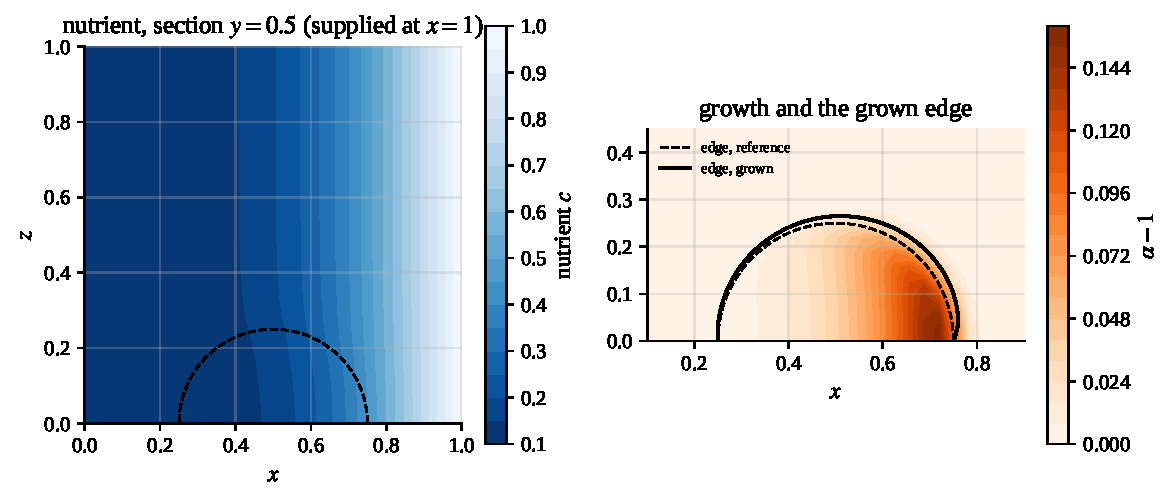
\includegraphics[width=0.85\linewidth]{fig_fuel_front_3d.pdf}\\
{\small 3D, section $y=0.5$: nutrient (left) and growth with the grown edge (right), $24^3$.}
\end{center}

\paragraph{3D with the five-species point model.} As above with the calibrated point model at
every node of the biofilm, $24^3$, $D=0.2$, $L_0=2$.
\begin{center}\small
\begin{tabularx}{\linewidth}{@{}Ycccc@{}}
\toprule
& living share, centre & $\alpha-1$, nutrient side / far side & edge $30^\circ$, nutrient side / far side\\
\midrule
no antibiotic & $0.518$ & $0.116$ / $0.005$ & $0.0186$ / $0.0047$\\
antibiotic, all species & $0.281$ & $0.086$ / $0.003$ & $0.0137$ / $0.0033$\\
antibiotic, anaerobes & $0.092$ & $0.057$ / $0.002$ & $0.0090$ / $0.0019$\\
\midrule
\multicolumn{4}{@{}l}{with the local nutrient in the point model (interaction $c^*c(\mathbf x)/c_{\rm ref}$, $c_{\rm ref}=1$):}\\
no antibiotic & $0.507$ & $0.135$ / $0.005$ & $0.0216$ / $0.0053$\\
antibiotic, all species & $0.332$ & $0.111$ / $0.004$ & $0.0176$ / $0.0043$\\
antibiotic, anaerobes & $0.354$ & $0.109$ / $0.004$ & $0.0174$ / $0.0044$\\
\bottomrule
\end{tabularx}
\end{center}
With the local nutrient the composition varies in space: on the nutrient side ($c=0.67$ for
$D=1$) \textit{V.~dispar} rises to $0.19$ and the living share falls to $0.37$, on the far side
($c=0.38$) they are $0.16$ and $0.44$; where the nutrient is scarce the interactions are weak and
more cells stay alive. The antibiotic reduces the edge displacement by $26\,\%$ (all species) and
$52\,\%$ (anaerobes) with the uniform interaction, by $19\,\%$ and $20\,\%$ with the local nutrient.
Field and point model share one time here ($T^*=1$ is Day~21 for both); the first 3D runs had
the point model only at about Day~5 and gave much weaker antibiotic effects.

\begin{center}
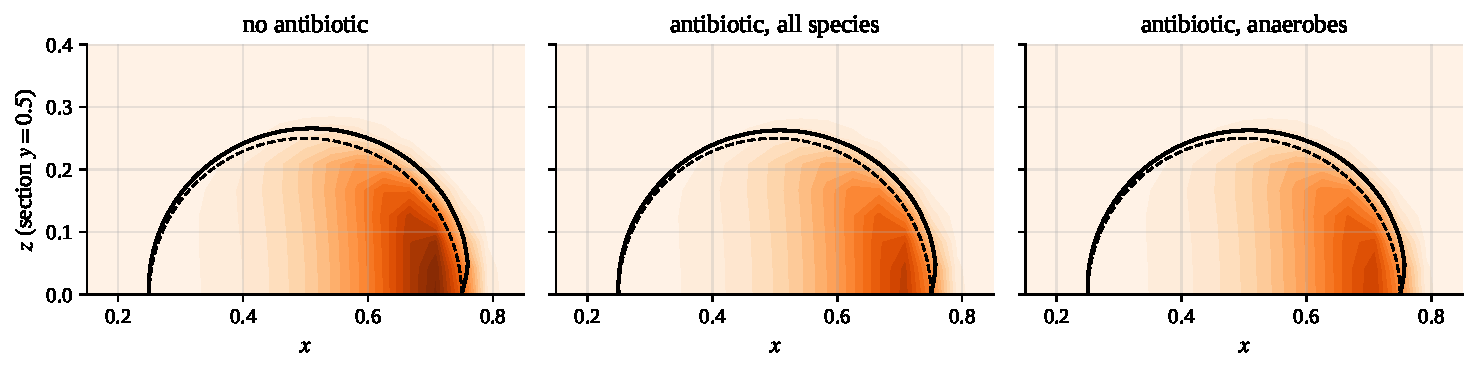
\includegraphics[width=\linewidth]{fig_fuel_front_3d_species_local.pdf}\\
{\small 3D, five species, local nutrient, section $y=0.5$: $\alpha-1$ and the grown edge
without antibiotic, with a broad antibiotic and with an anaerobe-specific one.}
\end{center}

\section{Finite element implementation}
\label{sec:fem}

The model is written as an Abaqus user element (\path{p3/uel/unified_uel.f90}): an 8-node
hexahedron with the displacement, $\phi$ and $c$ at the nodes (Abaqus degrees of freedom 1--3, 11,
12) and the composition, the growth $\xi=\alpha-1$ and a start flag at the $2\times2\times2$ Gauss
points. The phase and nutrient equations and the growth \eqref{eq:growth} are solved implicitly,
with the composition advanced once per increment by the point model of Klempt et al.\ 2026 at every
Gauss point where $\phi$ has passed $\phi_{\min}=0.05$ (staggered, the nutrient of the start of the
increment). The mechanics is finite strain, $\mathbf F=\mathbf F_e\mathbf F_g$,
$\mathbf F_g=\alpha\mathbf I$, with the energy per reference volume
\[W=\alpha^3(\phi^2+f)\Big[\frac{\mu}{2}\big(J_e^{-2/3}\,\mathbf I:\mathbf C_e-3\big)+\frac K2(J_e-1)^2\Big],\]
the mechanical term of Klempt et al.\ 2024 (Eq.~20) with a volumetric penalty in place of the
incompressibility constraint; small strain is an option. The tangent is written in closed form.
An antibiotic can be switched on at a given time through two element properties. The field and the
point model share one time: $T^*=1$ is Day~21 for both.

Abaqus is not available in the cloud; the element is checked by calling its entry point with
Abaqus's argument list (\path{p3/uel/emulate_abaqus.py}). The run inside Abaqus is the next step.

\begin{center}\small
\begin{tabularx}{\linewidth}{@{}Yp{5.2cm}@{}}
\toprule
check & result\\
\midrule
one element, uniform field: Gauss-point composition against the point model solved to convergence & $7.8\times10^{-16}$\\
1D column, 20 and 40 elements, against the 1D finite-difference model (Section~\ref{sec:results}) &
$\alpha-1$ $0.1371$ / $0.1370$ (1D: $0.137$), $\phi(0)$ $0.776$ / $0.772$ ($0.77$), $c(0)$ $0.936$ / $0.938$ ($0.938$)\\
repeated calls in one increment (as Abaqus iterates) & residual, tangent, state identical\\
closed-form tangent against central differences & $8.7\times10^{-10}$ (all rows), $7.2\times10^{-11}$
(mechanics, displacement gradients about $0.3$)\\
free growth $\mathbf u=(\alpha-1)\mathbf X$ & mechanics residual $2\times10^{-21}$\\
3D seed, $16^3$, small strain, against the finite-difference 3D model ($\lambda=0$) & $\phi$ at the
centre $0.778$ / $0.779$; edge $0.0135$ / $0.0126$; antibiotic $-23\,\%$ / $-24\,\%$\\
finite against small strain, $8^3$ & edge $0.0141$ against $0.0143$ ($\alpha-1\approx0.07$)\\
\bottomrule
\end{tabularx}
\end{center}

\paragraph{3D with the composition acting on the phase ($\lambda=1$).} Finite differences, $16^3$,
point model converged at every node and step. The absolute level of the point model's energy is
not fixed by the calibration (only its derivatives enter the point model), and with $\lambda>0$
it pushes the phase down: without a reference the biofilm shrinks by $16\,\%$ without antibiotic.
With the reference $\Psi_{\rm ref}=0.32$ (the time average of the untreated point model's energy)
the untreated biofilm stays near $\lambda=0$, and the antibiotic shrinks the biofilm itself.
\begin{center}\small
\begin{tabularx}{\linewidth}{@{}Yccc@{}}
\toprule
& biofilm volume (reference) & $\phi$, centre & edge $30^\circ$\\
\midrule
$\lambda=0$, no antibiotic & $0.0361$ & $0.78$ & $0.0126$\\
$\lambda=0$, antibiotic & $0.0361$ & $0.78$ & $0.0096$\\
$\lambda=1$, $\Psi_{\rm ref}=0.32$, no antibiotic & $0.0351$ & $0.78$ & $0.0115$\\
$\lambda=1$, $\Psi_{\rm ref}=0.32$, antibiotic & $0.0309$ ($-12\,\%$) & $0.67$ & $0.0083$\\
\bottomrule
\end{tabularx}
\end{center}
$\Psi_{\rm ref}$ is a new parameter, the energy of forming the biofilm; the time average is one
choice, and it should be fixed by the measured volume.

\section{Assumptions and open points}

\begin{center}\small
\begin{tabularx}{\linewidth}{@{}YYp{2.3cm}@{}}
\toprule
assumption & reason & tested\\
\midrule
two levels & one level fills the outer liquid (Section~\ref{sec:two}) & yes\\
weight $h(\phi)=\phi^2$ & with $h=\phi$ the composition force does not vanish in the outer
liquid and it fills again; $\phi^2$ is the weight of the mechanical term of Klempt et al.\ 2024 & yes\\
$\phi\le1$ by the one-sided barrier $K_\phi/(1-\phi)^2$ & the phase equation has no upper
bound (Klempt et al.\ 2024 neither); $\phi$ reached $2.7$ at large growth without it & yes\\
growth as a reaction with the living biomass as catalyst & Remark~\ref{rem:catalyst} & yes\\
ideal-solute energy of the nutrient, linear reaction kinetics & simplest forms consistent with
the principle & sensitivity only\\
$\lambda$, $\beta_s$, $L_0$, $Y$, $c_{\rm stop}$, $D$ & not from a paper; $\lambda$ sets how
strongly an antibiotic acts on the phase, $\beta_s$ does not matter for a seed & $\lambda$,
$\beta_s$ yes; others no\\
time link of the composition ($0.2375$ per $T^*$) & the calibration's; in the model it is the
ratio $\eta/\eta_\phi$ and can be fixed by the measured volume & no\\
local nutrient in the point model, $c^*c/c_{\rm ref}$ with $c_{\rm ref}=1$ & the element's
option; the relation of $c^*$ to $c$ should come from the nutrient level of the calibration & no\\
front term of Klempt et al.\ 2024 left out & not derivable from a potential; the edge moves by
the kinematics (Proposition~\ref{prop:front}) & 1D, 2D, 3D\\
mechanics: penalty in place of the incompressibility constraint, $\nu=0.3$ so far; nutrient in
the reference configuration & finite strain in the element (Section~\ref{sec:fem}); the
finite-difference 3D runs are small strain & finite against small strain\\
reference energy $\Psi_{\rm ref}$ for $\lambda>0$ & the calibration does not fix the level of the
point model's energy & one choice\\
\bottomrule
\end{tabularx}
\end{center}

\noindent Open: $\beta_s$ in 3D; $\nu=0.49$ in the element (locking of the 8-node hexahedron
needs an F-bar or mixed form); nutrient diffusion in the current configuration; the run inside
Abaqus; the limit $\phi\to0$ of the composition equations (regularised by
$\varepsilon$); existence and uniqueness (not attempted); a reader other than me; the overlap
with F.\ Klempt's unpublished two-species work (only published sources were used; to be
discussed before any publication). The checks establish that the equations are the ones the
energy and dissipation imply, that the solver solves them, and that the results do not depend
on the mesh or the time step at the level stated. They do not establish that the model is
right: the only data used are the calibrated interactions of the point model. The measured
volumes of Heine et al.\ and an antibiotic experiment would test the growth law and $\lambda$.
\end{document}
